\begin{center}

  \begin{tabular}{rp{16cm}lp{20cm}}%{rl}

  % after \\: \hline or \cline{col1-col2} \cline{col3-col4} ...

  论文地址:& \href{https://arxiv.org/pdf/1904.03751.pdf}{https://arxiv.org/pdf/1904.03751.pdf} \\
  来源:& ICCV, 2019\\
  作者:& Guohao Li, Matthias Muller, et al \\

  源码:& \href{https://github.com/lightaime/deep_gcns_torch}{deep\_gcns\_torch} \\

%  slides:& \href{http://yunshengb.com/wp-content/uploads/2017/03/nips_2018_r2l_workshop_talk.pdf}{{\footnotesize Convolutional Set Matching for Graph Similarity}}\\

  关键词:& \textbf{GCN, Point Cloud Segmentation} \\

  写于:& \date{2021-03-16}

  \end{tabular}

\end{center}

该论文\cite{li2019deepgcns}聚焦于深度GCN的训练及在点云数据上的分割问题。常见的GCN的层数都比较少,相关研究表明深层的GCN可能会引起如下问题:
\begin{itemize}
	\item over-smothing,一个连通分量内的结点的表征会趋同
	\item 较高的复杂度,不利于反向传播
	\item 梯度消失
\end{itemize}
该论文将CNN中的一些技巧引入深层GCN模型的构建,并将其应用在点云数据分割上。

\paragraph{问题定义}
\begin{figure}[h]
	\centering
	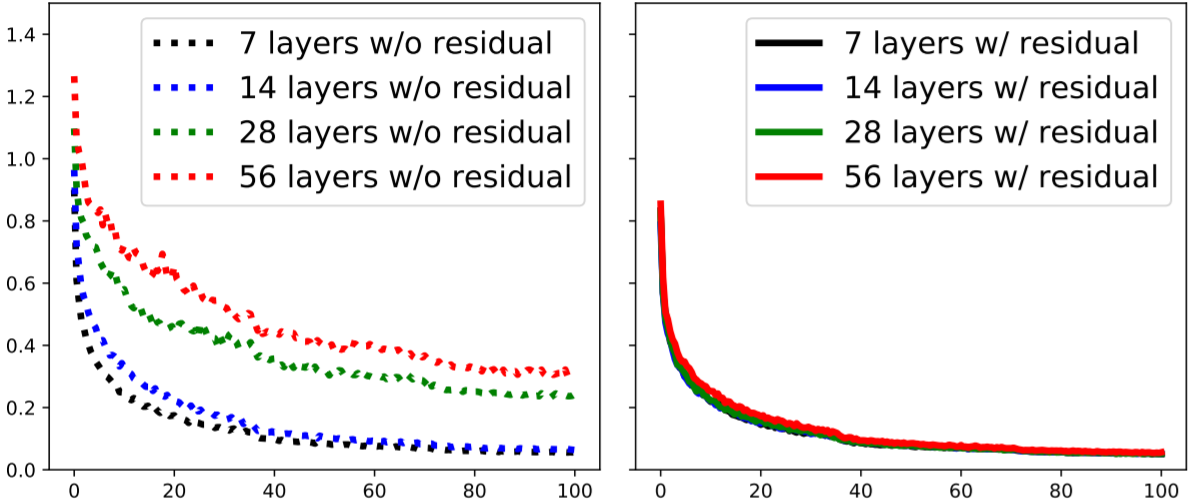
\includegraphics[width=.8\textwidth]{pics/Training-deep-GCNs.png}
	\caption{Traing deep GCNs}
	\label{fig:traing_deep_gcns}
\end{figure}
如Fig.\ref{fig:traing_deep_gcns}所示,当GCN的深度增加后,模型的损失并没有降低,这与\cite{he2016deep}中的模型退化现象很相似。怎么才可以让GCN像CNN一样,能够搭建出很深的模型呢?

\paragraph{DeepGCN}
作者从CNN中引入了三个技巧来解决这个问题:1)Residual learning;2)Dense Connection;3)Dilated Aggregation。

\subparagraph{Residual Learning for GCNs}
单纯地堆积卷积层对GCN地效果并没有很大的提升,其中一个原因可能是随着深度的增加,梯度难以反向传播,阻碍了模型的学习。Residual Learning的引入就是为了解决这个问题。
与Residual类似,如果原本要学习的映射为$\mathcal{H}$,残差的映射为$\mathcal{F}$,则残差学习表示如下:
$$
\begin{aligned}
	\mathcal{G}_{l+1} &= \mathcal{H}(\mathcal{G}_l, W_l)	\\
					  &= \mathcal{F}(\mathcal{G}_l, W_l) + \mathcal{G}_l = \mathcal{G}_{l+1}^{res} + \mathcal{G}_l
\end{aligned}
$$
第$l$层的输出经过$\mathcal{F}$的转换再与第$l$层的输出逐个顶点(vertex-wise)相加得到第$l+1$层的输出。

\subparagraph{Dense Connections in GCNs}
DenseNet的提出是为了利用层之间的稠密连接,提高网络中信息的流动,能够对层之间的特征进行重用,形式如下:
$$
\begin{aligned}
	\mathcal{G}_{l+1} &= \mathcal{H}(\mathcal{G}_l, W_l) \\
	  				  &= \mathcal{T}(\mathcal{F}(\mathcal{G}_l, W_l), \mathcal{G}_l) \\
	  				  &= \mathcal{T}(\mathcal{F}(\mathcal{G}_l, W_l), ..., \mathcal{F}(\mathcal{G}_0, W_0), \mathcal{G}_0)
\end{aligned}
$$
其中$\mathcal{T}$是一个逐顶点的连接操作,将输入的graph的结点的特征与中间各个GCN层的输出进行拼接。


\subparagraph{Dilated Aggregation inn GCNs}
空洞卷积弥补了pooling操作对空间信息的损失,在增大感受野的同时保留了位置信息。在改论文中,作者使用Dilated Aggregation来为每个结点聚集信息,以论文中进行的点云分割实验为例 --- 使用Dilated k-NN为每个顶点生成它的邻居。在每个GCN层后,作者使用Dilated k-NN来为每个顶点生成$k$个邻居,这$k$个邻居是从与这个顶点距离最近的$k \times d$个顶点以步长为$d$选择出来的,即顶点$v$的邻居为:$\mathcal{N}^{(d)}(v) = \{u_1, u_{1+d}, u_{1+2d}, ..., u_{1+(k-1)d}\}$。如Fig.\ref{fig:dilated_convolution_in_gcns}所示,上部分为dilated卷积,下部分为dilated k-NN,其中选择的$d$分别为1,2,4。在实践中,作者还增加了一点随机性,以$\epsilon$的概率随机从$k \times d$中选择$k$个顶点。

\begin{figure}[h]
	\centering
	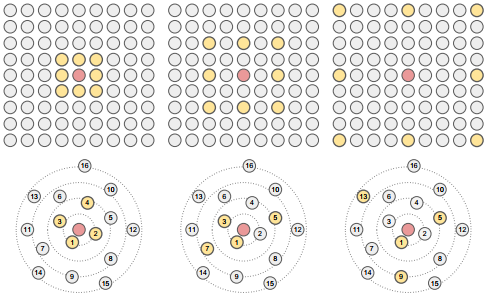
\includegraphics[width=.6\textwidth]{pics/Dilated-Convolution-in-GCNs.png}
	\caption{Dilated Convolution in  GCNs}
	\label{figz:dilated_convolution_in_gcns}
\end{figure}

最终,论文中用于点云数据分割的深度GCN架构如Fig.\ref{fig:deepgcn}所示。其中的区别为GCN Backbone Block,这个block有三个选择:1)普通的GCN;2)ResGCN;3)DenseGCN。
\begin{figure}[h]
	\centering
	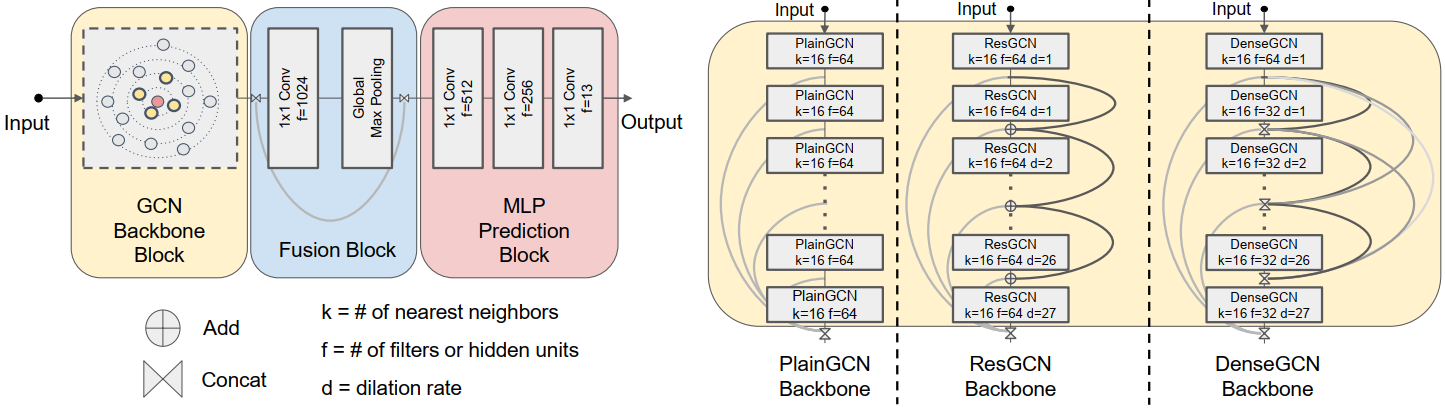
\includegraphics[width=.85\textwidth]{pics/DeepGCN.png}
	\caption{DeepGCN}
	\label{figz:deepgcn}
\end{figure}

\paragraph{总结}

\begin{itemize}

	\item 将CNN中的技术引入到GCN中,使得训练深层的GCN模型称为可能
	\item 将GCN应用于点云数据分割

\end{itemize}


%\paragraph{方法的局限性/未来方向}

%\begin{itemize}

%	\item 

%\end{itemize}




